%%%mark = star, diamond, square, otimes
%\documentclass{article}
%\usepackage{pgfplots}
%\usepackage[justification=centering]{caption}
%\pgfplotsset{compat=newest}
%\begin{document}
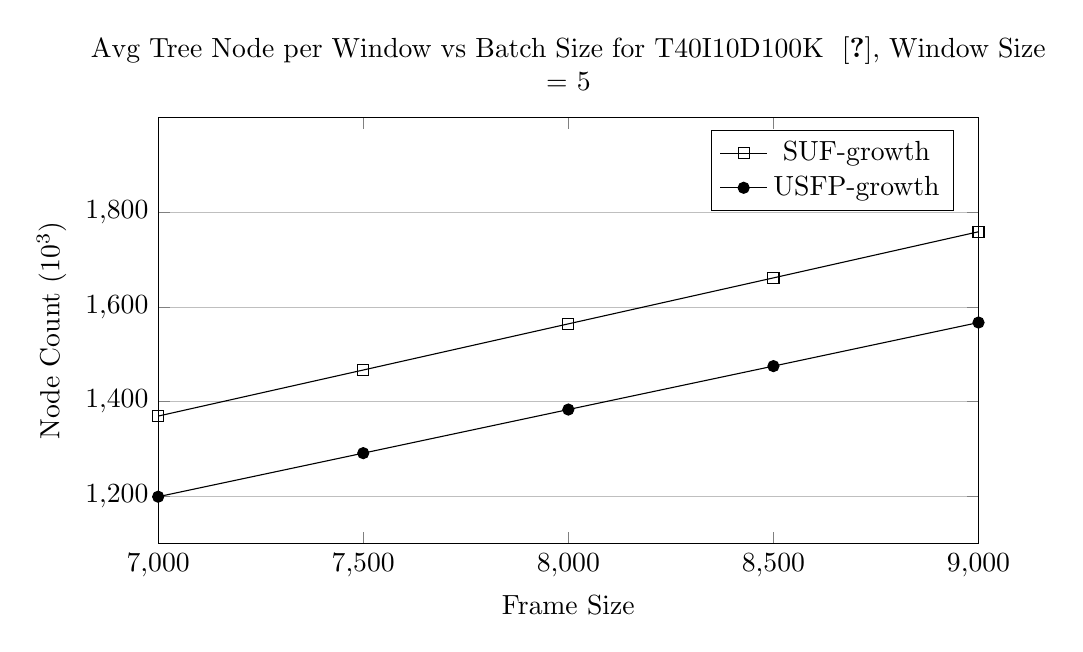
\begin{tikzpicture}
\begin{axis}[
	title={\parbox{\linewidth}{\centering Avg Tree Node per Window vs Batch Size for T40I10D100K ~\cite{dataset}, Window Size = 5}},
	width=12cm,
	height=7cm,
    xlabel={Frame Size },
    ylabel={Node Count ($10^3$)},
    xmin=7000, xmax=9000,
    ymin=1100, ymax=2000,
    xtick={7000,7500,8000,8500,9000},
    ytick={1200,1400,1600,1800},
    legend pos=north east,
    ymajorgrids=true,
    grid style={line width=.2pt,draw=gray!50},
]
 
\addplot[
    solid, every mark/.append style={solid, fill=gray}, mark=square
    ]
    coordinates {
			(7000,1369.555 )
			(7500,1466.766 )
			(8000,1564.122 )
			(8500,1661.100 )
			(9000,1758.412 )
			(9500,1855.734 )

	};
    \addlegendentry{SUF-growth}
\addplot[
    solid, every mark/.append style={solid, fill=black}, mark=*
    ]
    coordinates {
		(7000,1199.510)
		(7500,1291.388)
		(8000,1383.378)
		(8500,1474.984)
		(9000,1566.912)
		(9500,1658.773)

};
    \addlegendentry{USFP-growth}
 
\end{axis}
\end{tikzpicture}
%\end{document}